% ------------------------------------------------------------------------------------------------------------------
% Basic configuration and packages
% ------------------------------------------------------------------------------------------------------------------
% Package for discovering wrong and outdated usage of LaTeX.
% More information to be found in l2tabu English version.
\RequirePackage[l2tabu, orthodox]{nag}
% Class of LaTeX document: {size of paper, size of font}[document class]
\documentclass[a4paper,11pt]{article}



% ------------------------------------------------------
% Packages not tied to particular normal language
% ------------------------------------------------------
% This package should improved spaces in the text
\usepackage{microtype}
% Add few important symbols, like text Celcius degree
\usepackage{textcomp}



% ------------------------------------------------------
% Polonization of LaTeX document
% ------------------------------------------------------
% Basic polonization of the text
\usepackage[MeX]{polski}
% Switching on UTF-8 encoding
\usepackage[utf8]{inputenc}
% Adding font Latin Modern
\usepackage{lmodern}
% Package is need for fonts Latin Modern
\usepackage[T1]{fontenc}



% ------------------------------------------------------
% Setting margins
% ------------------------------------------------------
\usepackage[a4paper, total={14cm, 25cm}]{geometry}



% ------------------------------------------------------
% Setting vertical spaces in the text
% ------------------------------------------------------
% Setting space between lines
\renewcommand{\baselinestretch}{1.1}

% Setting space between lines in tables
\renewcommand{\arraystretch}{1.4}



% ------------------------------------------------------
% Packages for scientific papers
% ------------------------------------------------------
% Switching off \lll symbol, that I guess is representing letter "Ł"
% It collide with `amsmath' package's command with the same name
\let\lll\undefined
% Basic package from American Mathematical Society (AMS)
\usepackage[intlimits]{amsmath}
% Equations are numbered separately in every section
\numberwithin{equation}{section}

% Other very useful packages from AMS
\usepackage{amsfonts}
\usepackage{amssymb}
\usepackage{amscd}
\usepackage{amsthm}

% Package with better looking calligraphy fonts
\usepackage{calrsfs}

% Package with better looking greek letters
% Example of use: pi -> \uppi
\usepackage{upgreek}
% Improving look of lambda letter
\let\oldlambda\Lambda
\renewcommand{\lambda}{\uplambda}




% % ------------------------------------------------------
% % BibLaTeX
% % ------------------------------------------------------
% % Package biblatex, with biber as its backend, allow us to handle
% % bibliography entries that use Unicode symbols outside ASCII
% \usepackage[
% language=polish,
% backend=biber,
% style=alphabetic,
% url=false,
% eprint=true,
% ]{biblatex}

% \addbibresource{Logika-i-teoria-mnogości-Bibliography.bib}





% ------------------------------------------------------
% Defining new environments (?)
% ------------------------------------------------------
% Defining enviroment "Wniosek"
% \newtheorem{corollary}{Wniosek}
% \newtheorem{definition}{Definicja}
% \newtheorem{theorem}{Twierdzenie}





% ------------------------------------------------------
% Wonderful package PGF/TikZ
% ------------------------------------------------------
\usepackage{tikz}

% Loading TikZ libraries
% \usetikzlibrary{positioning}
% \usetikzlibrary{decorations.markings}

% Pics for drawing basic geometric objects
\usepackage{./Local-packages/PGF-TikZ-Geometry-pics}





% ------------------------------------------------------
% Local packages
% You need to put them in the same directory as .tex file
% ------------------------------------------------------
% Package containing various command useful for working with a text
% \usepackage{general-commands}
% Package containing commands and other code useful for working with
% mathematical text
% \usepackage{math-commands}





% ------------------------------------------------------
% Package "hyperref"
% They advised to put it on the end of preambule
% ------------------------------------------------------
% It allows you to use hyperlinks in the text
\usepackage{hyperref}










% ------------------------------------------------------------------------------------------------------------------
% Title and author of the text
\title{Figury geometryczne na płaszczyźnie \\
  {\Large Rysunki i~wykresy}}

\author{Kamil Ziemian}


% \date{}
% ------------------------------------------------------------------------------------------------------------------










% ####################################################################
% Beginning of the document
\begin{document}
% ####################################################################





% ######################################
% Title of the text
\maketitle
% ######################################





% ##################
\begin{figure}

  \label{fig:Okregi}


  \centering

  \begin{tikzpicture}

    % Center of circles
    \pic at (0,0) {point};



    % ############################
    % Circles
    \draw (0,0) circle [radius=1];

    \node at (0,-1.275) {$r = 1$};



    \draw (0,0) circle [radius=2];

    \node at (0,-2.275) {$r = 2$};



    \draw (0,0) circle [radius=3];

    \node at (0,-3.275) {$r = 3$};



    \draw (0,0) circle [radius=4];

    \node at (0,-4.275) {$r = 4$};

  \end{tikzpicture}

  \caption{Okręgi}

\end{figure}
% ##################





% ##################
\begin{figure}

  \label{fig:Elipsy-01}


  \centering

  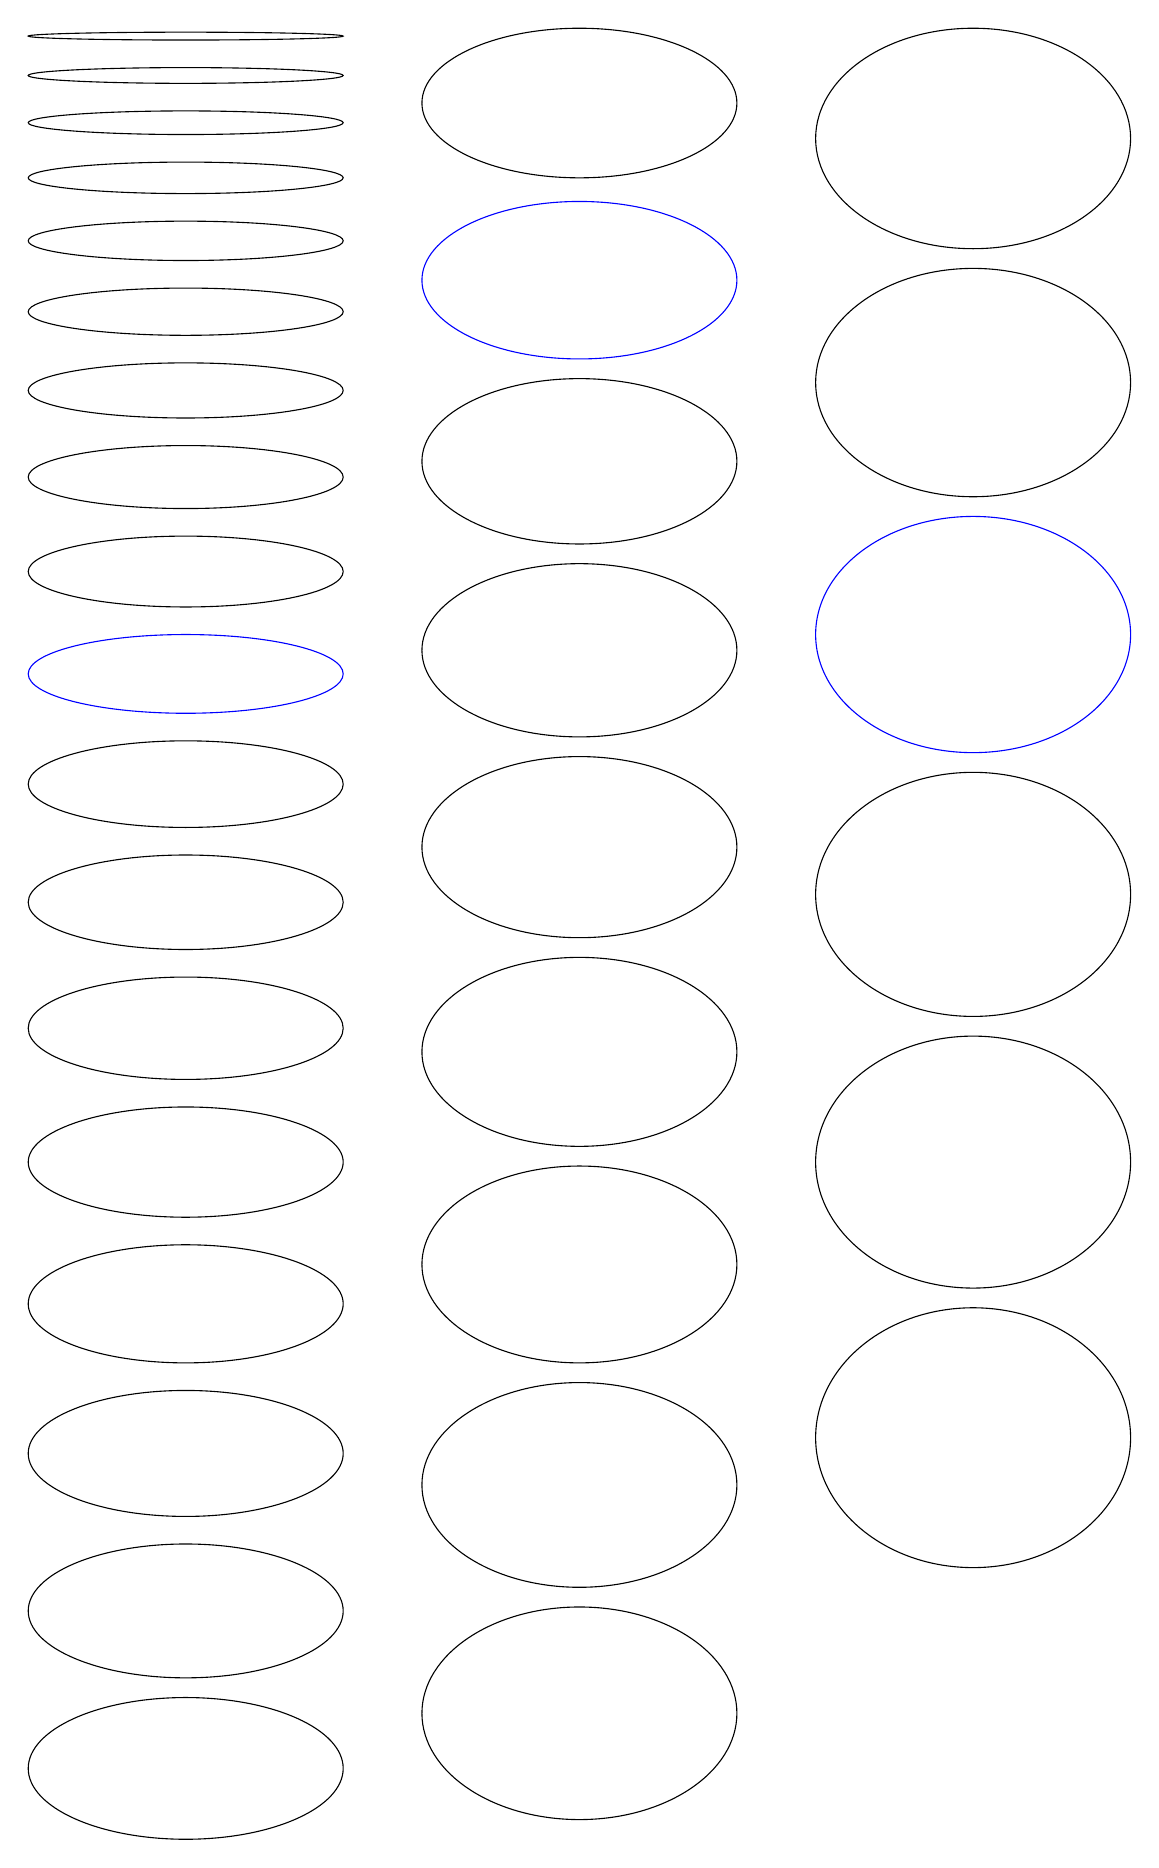
\begin{tikzpicture}

    \draw (0,0) ellipse [x radius=2, y radius=0.05];



    \begin{scope}[yshift=-0.5cm]

      \draw (0,0) ellipse [x radius=2, y radius=0.1];

    \end{scope}



    \begin{scope}[yshift=-1.1cm]

      \draw (0,0) ellipse [x radius=2, y radius=0.15];

    \end{scope}



    \begin{scope}[yshift=-1.8cm]

      \draw (0,0) ellipse [x radius=2, y radius=0.2];

    \end{scope}



    \begin{scope}[yshift=-2.6cm]

      \draw (0,0) ellipse [x radius=2, y radius=0.25];

    \end{scope}



    \begin{scope}[yshift=-3.5cm]

      \draw (0,0) ellipse [x radius=2, y radius=0.3];

    \end{scope}



    \begin{scope}[yshift=-4.5cm]

      \draw (0,0) ellipse [x radius=2, y radius=0.35];

    \end{scope}



    \begin{scope}[yshift=-5.6cm]

      \draw (0,0) ellipse [x radius=2, y radius=0.4];

    \end{scope}



    \begin{scope}[yshift=-6.8cm]

      \draw (0,0) ellipse [x radius=2, y radius=0.45];

    \end{scope}



    \begin{scope}[yshift=-8.1cm]

      \draw[color=blue] (0,0) ellipse [x radius=2, y radius=0.5];

    \end{scope}



    \begin{scope}[yshift=-9.5cm]

      \draw (0,0) ellipse [x radius=2, y radius=0.55];

    \end{scope}



    \begin{scope}[yshift=-11cm]

      \draw (0,0) ellipse [x radius=2, y radius=0.6];

    \end{scope}



    \begin{scope}[yshift=-12.6cm]

      \draw (0,0) ellipse [x radius=2, y radius=0.65];

    \end{scope}



    \begin{scope}[yshift=-14.3cm]

      \draw (0,0) ellipse [x radius=2, y radius=0.7];

    \end{scope}



    \begin{scope}[yshift=-16.1cm]

      \draw (0,0) ellipse [x radius=2, y radius=0.75];

    \end{scope}



    \begin{scope}[yshift=-18cm]

      \draw (0,0) ellipse [x radius=2, y radius=0.8];

    \end{scope}



    \begin{scope}[yshift=-20cm]

      \draw (0,0) ellipse [x radius=2, y radius=0.85];

    \end{scope}



    \begin{scope}[yshift=-22cm]

      \draw (0,0) ellipse [x radius=2, y radius=0.9];

    \end{scope}










    \begin{scope}[xshift=5cm,yshift=-0.85cm]

      \draw (0,0) ellipse [x radius=2, y radius=0.95];

    \end{scope}



    \begin{scope}[xshift=5cm,yshift=-3.1cm]

      \draw[color=blue] (0,0) ellipse [x radius=2, y radius=1];

    \end{scope}



    \begin{scope}[xshift=5cm,yshift=-5.4cm]

      \draw (0,0) ellipse [x radius=2, y radius=1.05];

    \end{scope}




    \begin{scope}[xshift=5cm,yshift=-7.8cm]

      \draw (0,0) ellipse [x radius=2, y radius=1.1];

    \end{scope}




    \begin{scope}[xshift=5cm,yshift=-10.3cm]

      \draw (0,0) ellipse [x radius=2, y radius=1.15];

    \end{scope}



    \begin{scope}[xshift=5cm,yshift=-12.9cm]

      \draw (0,0) ellipse [x radius=2, y radius=1.2];

    \end{scope}



    \begin{scope}[xshift=5cm,yshift=-15.6cm]

      \draw (0,0) ellipse [x radius=2, y radius=1.25];

    \end{scope}



    \begin{scope}[xshift=5cm,yshift=-18.4cm]

      \draw (0,0) ellipse [x radius=2, y radius=1.3];

    \end{scope}



    \begin{scope}[xshift=5cm,yshift=-21.3cm]

      \draw (0,0) ellipse [x radius=2, y radius=1.35];

    \end{scope}










    \begin{scope}[xshift=10cm,yshift=-1.3cm]

      \draw (0,0) ellipse [x radius=2, y radius=1.4];

    \end{scope}



    \begin{scope}[xshift=10cm,yshift=-4.4cm]

      \draw (0,0) ellipse [x radius=2, y radius=1.45];

    \end{scope}



    \begin{scope}[xshift=10cm,yshift=-7.6cm]

      \draw[color=blue] (0,0) ellipse [x radius=2, y radius=1.5];

    \end{scope}



    \begin{scope}[xshift=10cm,yshift=-10.9cm]

      \draw (0,0) ellipse [x radius=2, y radius=1.55];

    \end{scope}



    \begin{scope}[xshift=10cm,yshift=-14.3cm]

      \draw (0,0) ellipse [x radius=2, y radius=1.6];

    \end{scope}



    \begin{scope}[xshift=10cm,yshift=-17.8cm]

      \draw (0,0) ellipse [x radius=2, y radius=1.65];

    \end{scope}

  \end{tikzpicture}

  \caption{Elipsy~1}


\end{figure}
% ##################





% ##################
\begin{figure}

  \label{fig:Elipsy-02}


  \centering

  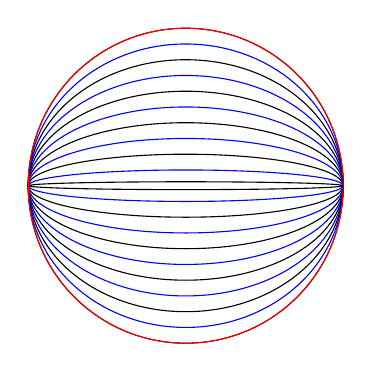
\begin{tikzpicture}

    \draw (0,0) ellipse [x radius=2, y radius=0.05];

    \draw[color=blue] (0,0) ellipse [x radius=2, y radius=0.2];

    \draw (0,0) ellipse [x radius=2, y radius=0.4];

    \draw[color=blue] (0,0) ellipse [x radius=2, y radius=0.6];

    \draw (0,0) ellipse [x radius=2, y radius=0.8];

    \draw[color=blue] (0,0) ellipse [x radius=2, y radius=1];

    \draw (0,0) ellipse [x radius=2, y radius=1.2];

    \draw[color=blue] (0,0) ellipse [x radius=2, y radius=1.4];

    \draw (0,0) ellipse [x radius=2, y radius=1.6];

    \draw[color=blue] (0,0) ellipse [x radius=2, y radius=1.8];

    \draw (0,0) ellipse [x radius=2, y radius=2];




    \draw[color=red] (0,0) ellipse [x radius=2, y radius=2];

  \end{tikzpicture}

  \caption{Elipsy~2}


\end{figure}
% ##################





% ##################
\begin{figure}

  \label{fig:Elipsy-03}


  \centering

  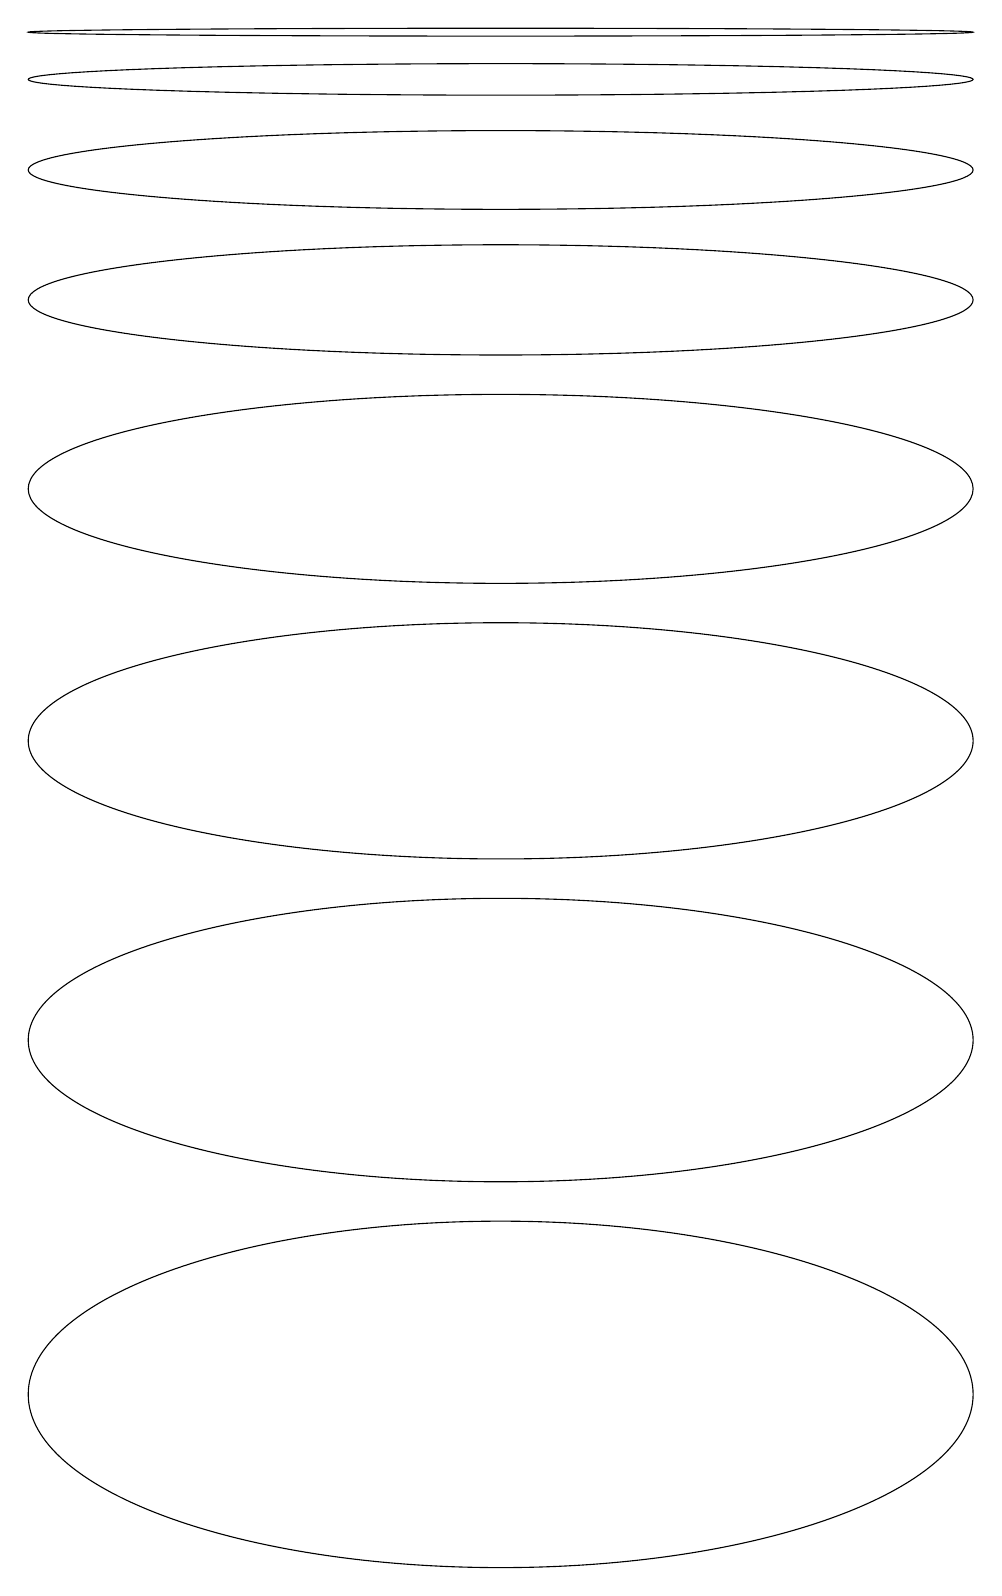
\begin{tikzpicture}

    \draw (0,0) ellipse [x radius=6, y radius=0.05];



    \begin{scope}[yshift=-0.6cm]

      \draw (0,0) ellipse [x radius=6, y radius=0.2];

    \end{scope}



    \begin{scope}[yshift=-1.75cm]

      \draw (0,0) ellipse [x radius=6, y radius=0.5];

    \end{scope}



    \begin{scope}[yshift=-3.4cm]

      \draw (0,0) ellipse [x radius=6, y radius=0.7];

    \end{scope}



    \begin{scope}[yshift=-5.8cm]

      \draw (0,0) ellipse [x radius=6, y radius=1.2];

    \end{scope}



    \begin{scope}[yshift=-9cm]

      \draw (0,0) ellipse [x radius=6, y radius=1.5];

    \end{scope}



    \begin{scope}[yshift=-12.8cm]

      \draw (0,0) ellipse [x radius=6, y radius=1.8];

    \end{scope}



    \begin{scope}[yshift=-17.3cm]

      \draw (0,0) ellipse [x radius=6, y radius=2.2];

    \end{scope}

  \end{tikzpicture}

  \caption{Elipsy~3}


\end{figure}
% ##################





% ##################
\begin{figure}

  \label{fig:Elipsy-04}


  \centering

  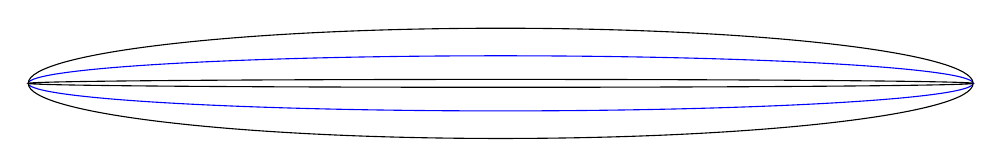
\begin{tikzpicture}

    \draw (0,0) ellipse [x radius=6, y radius=0.05];

    \draw[color=blue] (0,0) ellipse [x radius=6, y radius=0.35];

    \draw (0,0) ellipse [x radius=6, y radius=0.7];

  \end{tikzpicture}

  \caption{Elipsy~4}


\end{figure}
% ##################





% ##################
\begin{figure}

  \label{fig:Elipsy-05}


  \centering

  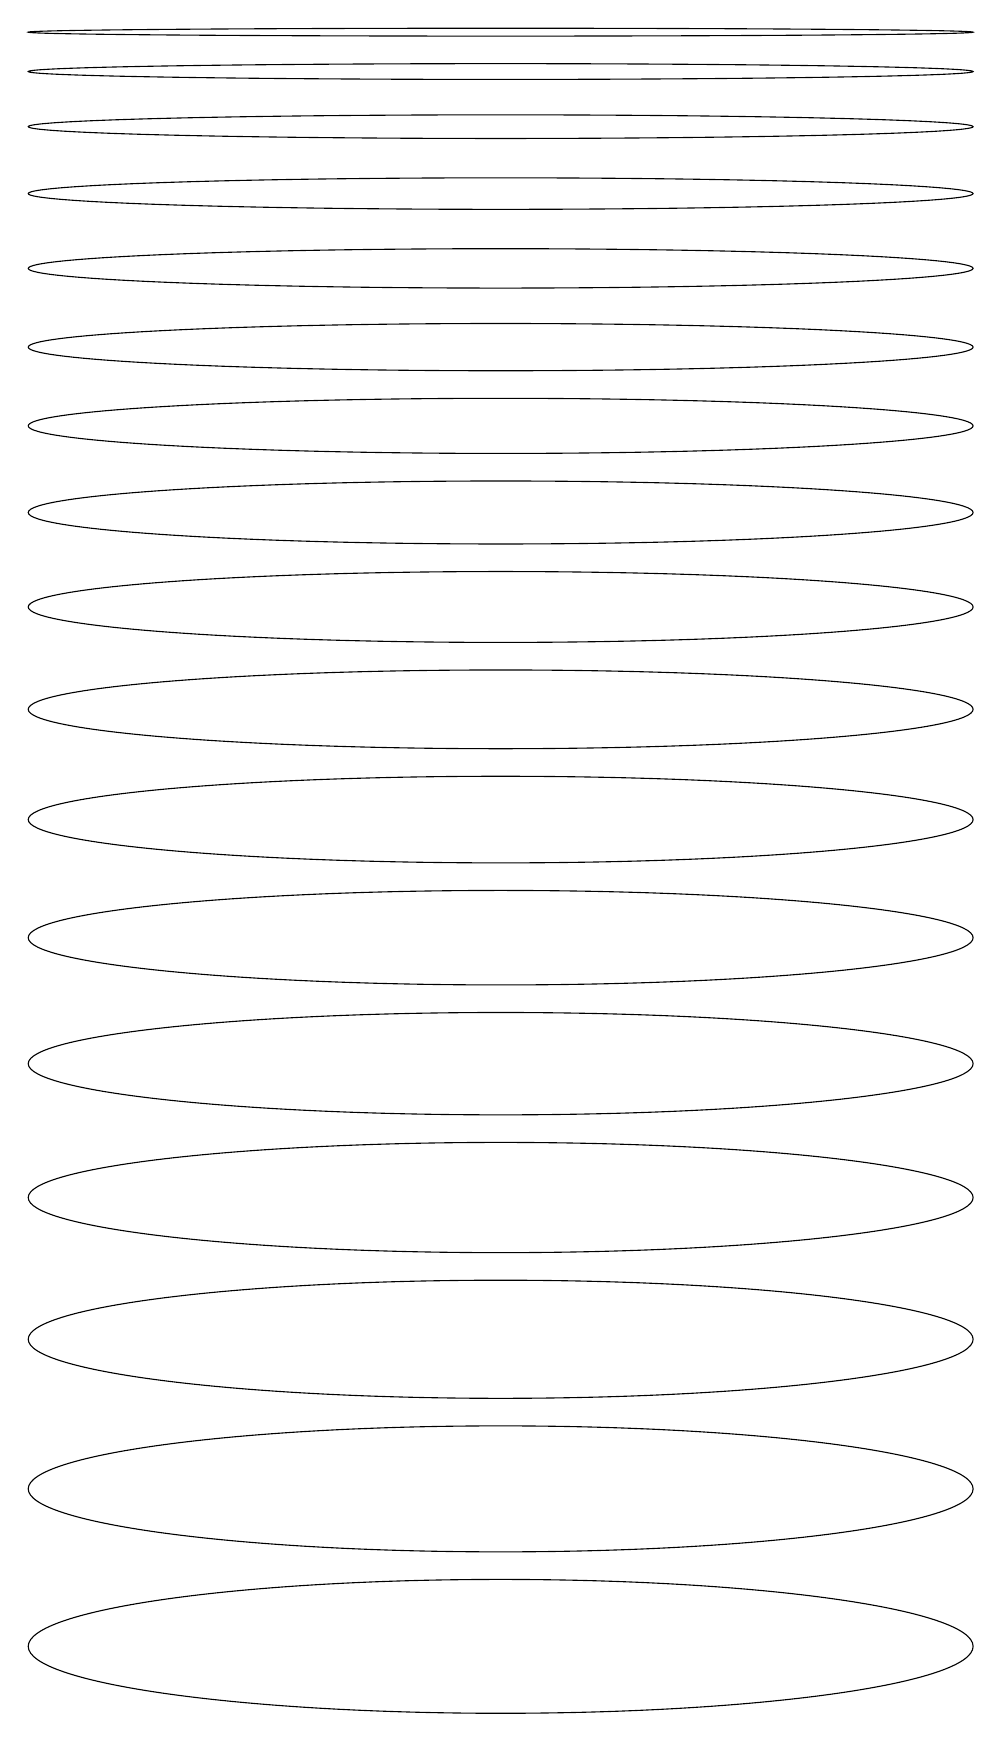
\begin{tikzpicture}

    \draw (0,0) ellipse [x radius=6, y radius=0.05];



    \begin{scope}[yshift=-0.5cm]

      \draw (0,0) ellipse [x radius=6, y radius=0.1];

    \end{scope}



    \begin{scope}[yshift=-1.2cm]

      \draw (0,0) ellipse [x radius=6, y radius=0.15];

    \end{scope}



    \begin{scope}[yshift=-2.05cm]

      \draw (0,0) ellipse [x radius=6, y radius=0.2];

    \end{scope}



    \begin{scope}[yshift=-3cm]

      \draw (0,0) ellipse [x radius=6, y radius=0.25];

    \end{scope}



    \begin{scope}[yshift=-4cm]

      \draw (0,0) ellipse [x radius=6, y radius=0.3];

    \end{scope}



    \begin{scope}[yshift=-5cm]

      \draw (0,0) ellipse [x radius=6, y radius=0.35];

    \end{scope}



    \begin{scope}[yshift=-6.1cm]

      \draw (0,0) ellipse [x radius=6, y radius=0.4];

    \end{scope}



    \begin{scope}[yshift=-7.3cm]

      \draw (0,0) ellipse [x radius=6, y radius=0.45];

    \end{scope}



    \begin{scope}[yshift=-8.6cm]

      \draw (0,0) ellipse [x radius=6, y radius=0.5];

    \end{scope}



    \begin{scope}[yshift=-10cm]

      \draw (0,0) ellipse [x radius=6, y radius=0.55];

    \end{scope}



    \begin{scope}[yshift=-11.5cm]

      \draw (0,0) ellipse [x radius=6, y radius=0.6];

    \end{scope}



    \begin{scope}[yshift=-13.1cm]

      \draw (0,0) ellipse [x radius=6, y radius=0.65];

    \end{scope}



    \begin{scope}[yshift=-14.8cm]

      \draw (0,0) ellipse [x radius=6, y radius=0.7];

    \end{scope}



    \begin{scope}[yshift=-16.6cm]

      \draw (0,0) ellipse [x radius=6, y radius=0.75];

    \end{scope}



    \begin{scope}[yshift=-18.5cm]

      \draw (0,0) ellipse [x radius=6, y radius=0.8];

    \end{scope}



    \begin{scope}[yshift=-20.5cm]

      \draw (0,0) ellipse [x radius=6, y radius=0.85];

    \end{scope}

  \end{tikzpicture}

  \caption{Elipsy~5}


\end{figure}
% ##################





% ##################
\begin{figure}

  \label{fig:Elipsy-06}


  \centering

  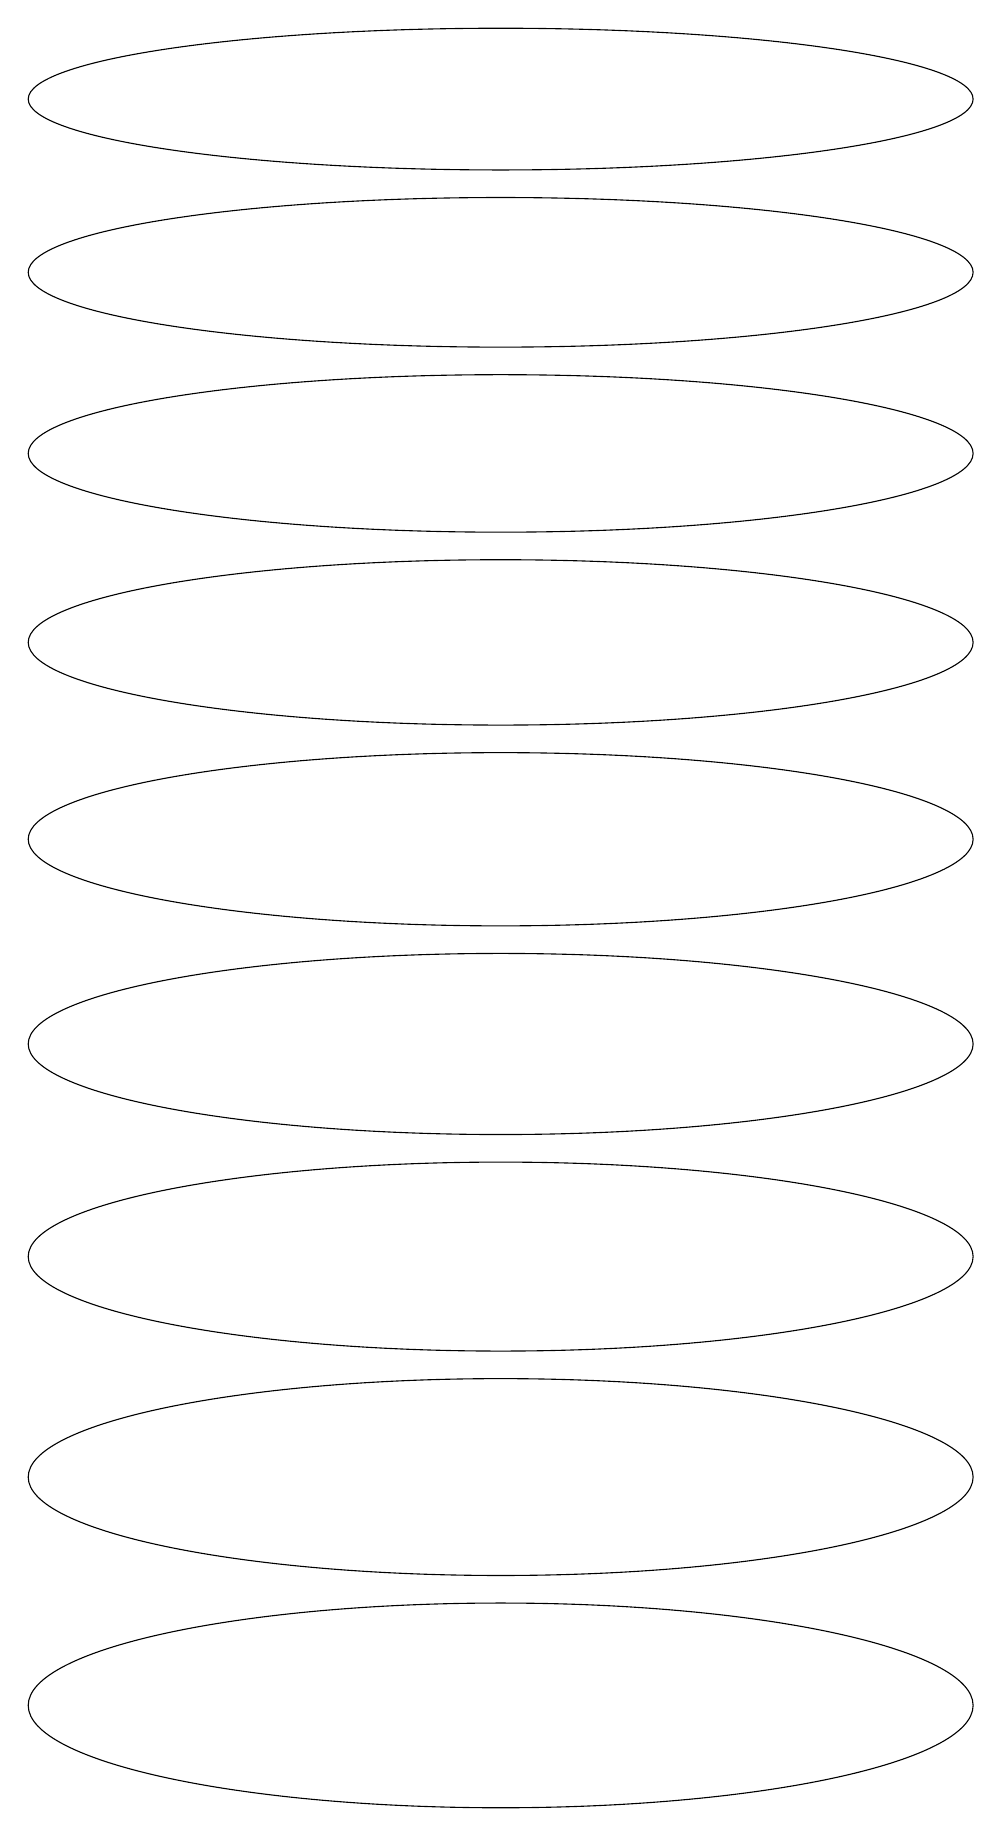
\begin{tikzpicture}

    \draw (0,0) ellipse [x radius=6, y radius=0.9];



    \begin{scope}[yshift=-2.2cm]

      \draw (0,0) ellipse [x radius=6, y radius=0.95];

    \end{scope}



    \begin{scope}[yshift=-4.5cm]

      \draw (0,0) ellipse [x radius=6, y radius=1];

    \end{scope}



    \begin{scope}[yshift=-6.9cm]

      \draw (0,0) ellipse [x radius=6, y radius=1.05];

    \end{scope}



    \begin{scope}[yshift=-9.4cm]

      \draw (0,0) ellipse [x radius=6, y radius=1.1];

    \end{scope}



    \begin{scope}[yshift=-12cm]

      \draw (0,0) ellipse [x radius=6, y radius=1.15];

    \end{scope}



    \begin{scope}[yshift=-14.7cm]

      \draw (0,0) ellipse [x radius=6, y radius=1.2];

    \end{scope}



    \begin{scope}[yshift=-17.5cm]

      \draw (0,0) ellipse [x radius=6, y radius=1.25];

    \end{scope}



    \begin{scope}[yshift=-20.4cm]

      \draw (0,0) ellipse [x radius=6, y radius=1.3];

    \end{scope}

  \end{tikzpicture}

  \caption{Elipsy~6}


\end{figure}
% ##################





% ##################
\begin{figure}

  \label{fig:Elipsy-07}


  \centering

  \begin{tikzpicture}

    \draw (0,0) ellipse [x radius=6, y radius=1.35];



    \begin{scope}[yshift=-3.1cm]

      \draw (0,0) ellipse [x radius=6, y radius=1.4];

    \end{scope}



    \begin{scope}[yshift=-6.3cm]

      \draw (0,0) ellipse [x radius=6, y radius=1.45];

    \end{scope}



    \begin{scope}[yshift=-9.6cm]

      \draw (0,0) ellipse [x radius=6, y radius=1.5];

    \end{scope}



    \begin{scope}[yshift=-13cm]

      \draw (0,0) ellipse [x radius=6, y radius=1.55];

    \end{scope}



    \begin{scope}[yshift=-16.5cm]

      \draw (0,0) ellipse [x radius=6, y radius=1.6];

    \end{scope}



    \begin{scope}[yshift=-20.1cm]

      \draw (0,0) ellipse [x radius=6, y radius=1.65];

    \end{scope}

  \end{tikzpicture}

  \caption{Elipsy~7}


\end{figure}
% ##################





% ##################
\begin{figure}

  \label{fig:Elipsy-08}


  \centering

  \begin{tikzpicture}

    \draw (0,0) ellipse [x radius=6, y radius=1.7];



    \begin{scope}[yshift=-3.9cm]

      \draw (0,0) ellipse [x radius=6, y radius=1.75];

    \end{scope}



    \begin{scope}[yshift=-7.9cm]

      \draw (0,0) ellipse [x radius=6, y radius=1.8];

    \end{scope}



    \begin{scope}[yshift=-12cm]

      \draw (0,0) ellipse [x radius=6, y radius=1.85];

    \end{scope}



    \begin{scope}[yshift=-16.2cm]

      \draw (0,0) ellipse [x radius=6, y radius=1.9];

    \end{scope}



    \begin{scope}[yshift=-20.4cm]

      \draw (0,0) ellipse [x radius=6, y radius=1.95];

    \end{scope}

  \end{tikzpicture}

  \caption{Elipsy~8}


\end{figure}
% ##################





% ##################
\begin{figure}

  \label{fig:Elipsy-09}


  \centering

  \begin{tikzpicture}

    \draw (0,0) ellipse [x radius=6, y radius=2];



    \begin{scope}[yshift=-4.5cm]

      \draw (0,0) ellipse [x radius=6, y radius=2.05];

    \end{scope}



    \begin{scope}[yshift=-9.1cm]

      \draw (0,0) ellipse [x radius=6, y radius=2.1];

    \end{scope}



    \begin{scope}[yshift=-13.8cm]

      \draw (0,0) ellipse [x radius=6, y radius=2.15];

    \end{scope}



    \begin{scope}[yshift=-18.5cm]

      \draw (0,0) ellipse [x radius=6, y radius=2.2];

    \end{scope}

  \end{tikzpicture}

  \caption{Elipsy~9}


\end{figure}
% ##################





% ##################
\begin{figure}

  \label{fig:Elipsy-10}


  \centering

  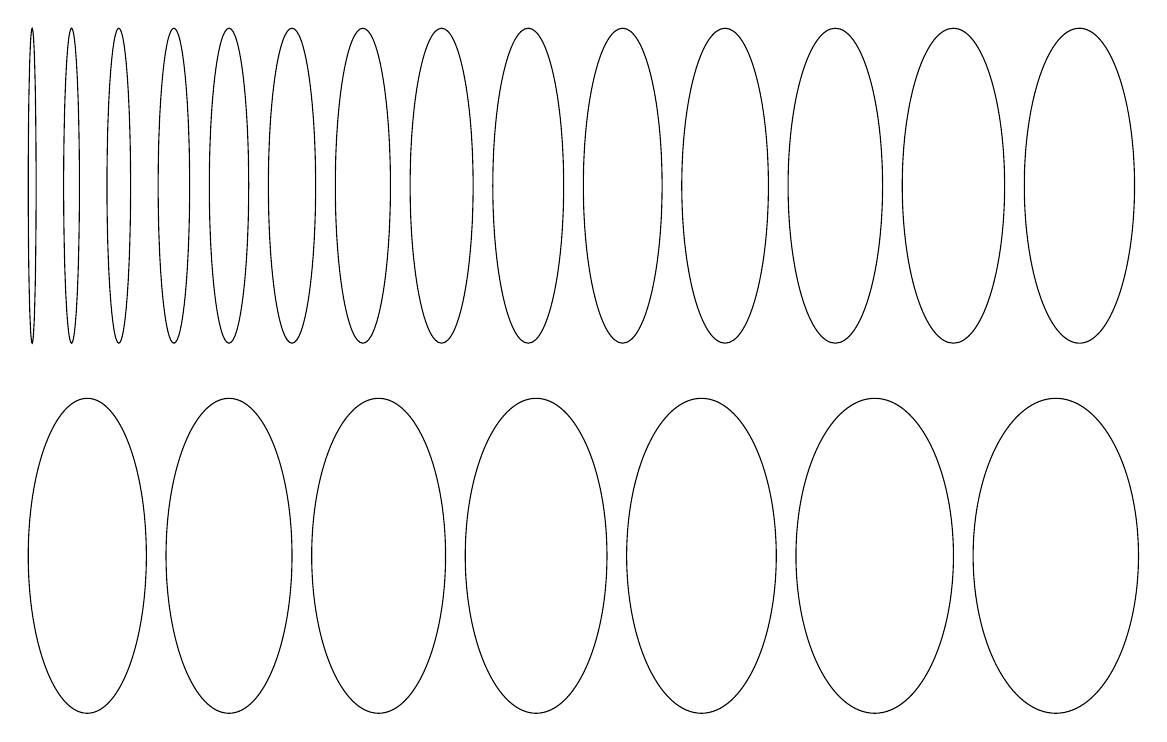
\begin{tikzpicture}

    \draw (0,0) ellipse [x radius=0.05, y radius=2];




    \begin{scope}[xshift=0.5cm]

      \draw (0,0) ellipse [x radius=0.1, y radius=2];

    \end{scope}



    \begin{scope}[xshift=1.1cm]

      \draw (0,0) ellipse [x radius=0.15, y radius=2];

    \end{scope}



    \begin{scope}[xshift=1.8cm]

      \draw (0,0) ellipse [x radius=0.2, y radius=2];

    \end{scope}



    \begin{scope}[xshift=2.5cm]

      \draw (0,0) ellipse [x radius=0.25, y radius=2];

    \end{scope}



    \begin{scope}[xshift=3.3cm]

      \draw (0,0) ellipse [x radius=0.3, y radius=2];

    \end{scope}



    \begin{scope}[xshift=4.2cm]

      \draw (0,0) ellipse [x radius=0.35, y radius=2];

    \end{scope}



    \begin{scope}[xshift=5.2cm]

      \draw (0,0) ellipse [x radius=0.4, y radius=2];

    \end{scope}



    \begin{scope}[xshift=6.3cm]

      \draw (0,0) ellipse [x radius=0.45, y radius=2];

    \end{scope}



    \begin{scope}[xshift=7.5cm]

      \draw (0,0) ellipse [x radius=0.5, y radius=2];

    \end{scope}



    \begin{scope}[xshift=8.8cm]

      \draw (0,0) ellipse [x radius=0.55, y radius=2];

    \end{scope}



    \begin{scope}[xshift=10.2cm]

      \draw (0,0) ellipse [x radius=0.6, y radius=2];

    \end{scope}




    \begin{scope}[xshift=11.7cm]

      \draw (0,0) ellipse [x radius=0.65, y radius=2];

    \end{scope}




    \begin{scope}[xshift=13.3cm]

      \draw (0,0) ellipse [x radius=0.7, y radius=2];

    \end{scope}










    \begin{scope}[xshift=0.7cm,yshift=-4.7cm]

      \draw (0,0) ellipse [x radius=0.75, y radius=2];

    \end{scope}



    \begin{scope}[xshift=2.5cm,yshift=-4.7cm]

      \draw (0,0) ellipse [x radius=0.8, y radius=2];

    \end{scope}



    \begin{scope}[xshift=4.4cm,yshift=-4.7cm]

      \draw (0,0) ellipse [x radius=0.85, y radius=2];

    \end{scope}



    \begin{scope}[xshift=6.4cm,yshift=-4.7cm]

      \draw (0,0) ellipse [x radius=0.9, y radius=2];

    \end{scope}



    \begin{scope}[xshift=8.5cm,yshift=-4.7cm]

      \draw (0,0) ellipse [x radius=0.95, y radius=2];

    \end{scope}



    \begin{scope}[xshift=10.7cm,yshift=-4.7cm]

      \draw (0,0) ellipse [x radius=1, y radius=2];

    \end{scope}



    \begin{scope}[xshift=13cm,yshift=-4.7cm]

      \draw (0,0) ellipse [x radius=1.05, y radius=2];

    \end{scope}

  \end{tikzpicture}

  \caption{Elipsy~10}



\end{figure}
% ##################





% ##################
\begin{figure}

  \label{fig:Elipsy-11}


  \centering

  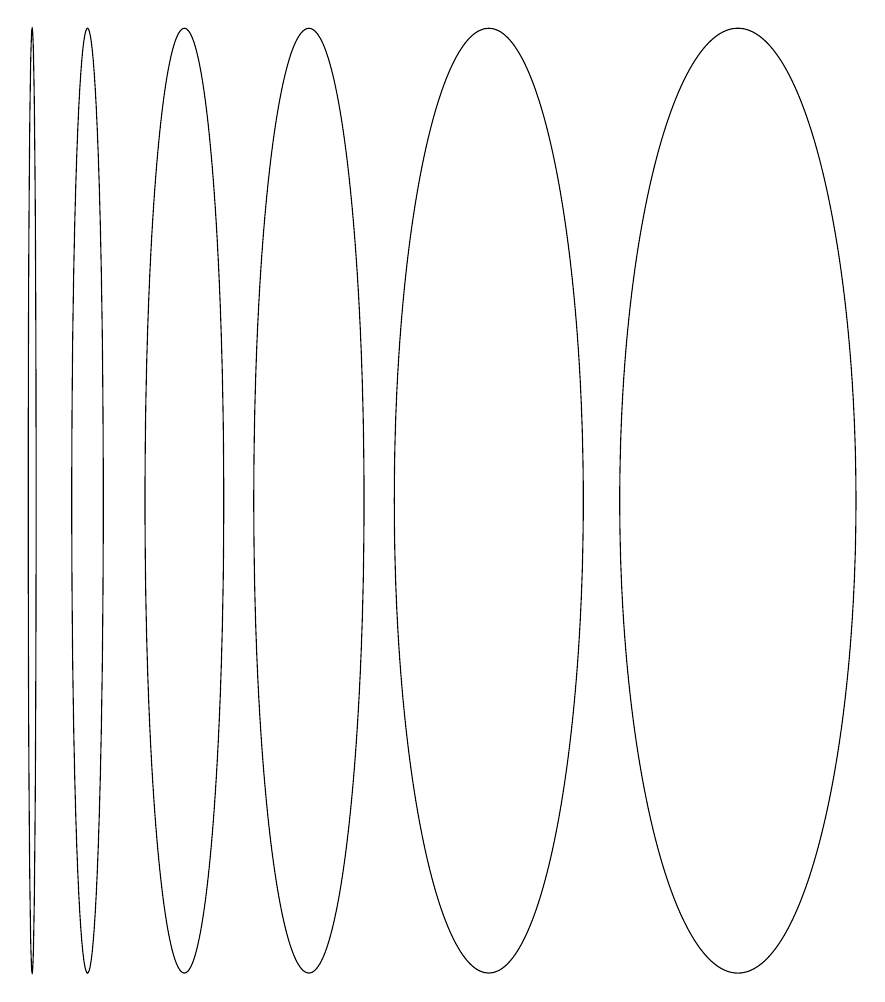
\begin{tikzpicture}

    \draw (0,0) ellipse [x radius=0.05, y radius=6];




    \begin{scope}[xshift=20]

      \draw (0,0) ellipse [x radius=0.2, y radius=6];

    \end{scope}



    \begin{scope}[xshift=55]

      \draw (0,0) ellipse [x radius=0.5, y radius=6];

    \end{scope}



    \begin{scope}[xshift=100]

      \draw (0,0) ellipse [x radius=0.7, y radius=6];

    \end{scope}



    \begin{scope}[xshift=165]

      \draw (0,0) ellipse [x radius=1.2, y radius=6];

    \end{scope}



    \begin{scope}[xshift=255]

      \draw (0,0) ellipse [x radius=1.5, y radius=6];

    \end{scope}

  \end{tikzpicture}

  \caption{Elipsy~11}

\end{figure}
% ##################





% ##################
\begin{figure}

  \label{fig:Elipsy-12}


  \centering

  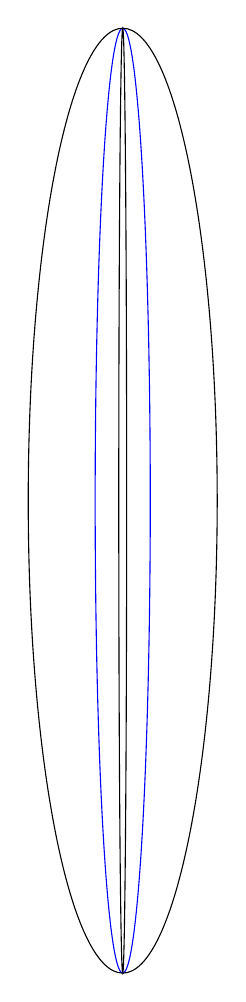
\begin{tikzpicture}

    \draw (0,0) ellipse [x radius=0.05, y radius=6];

    \draw[color=blue] (0,0) ellipse [x radius=0.35, y radius=6];

    \draw (0,0) ellipse [x radius=1.2, y radius=6];

  \end{tikzpicture}

  \caption{Elipsy~12}


\end{figure}
% ##################























































% ####################################################################
% ####################################################################
% Bibliography

% \printbibliography





% ############################
% End of the document

\end{document}
